\newpage
\section{Versuchsdurchführung}

\subsection*{Aufbau}
Der Versuchsaufbau ist schematisch in Abb. \ref{fig:fliessbild} als Verfahrensfließbild dargestellt. Zu beachten ist, dass die Regelung für den Heizlüfter  in dieser Darstellung nicht aufgeführt ist.

\begin{figure}[h!]
	\centering
	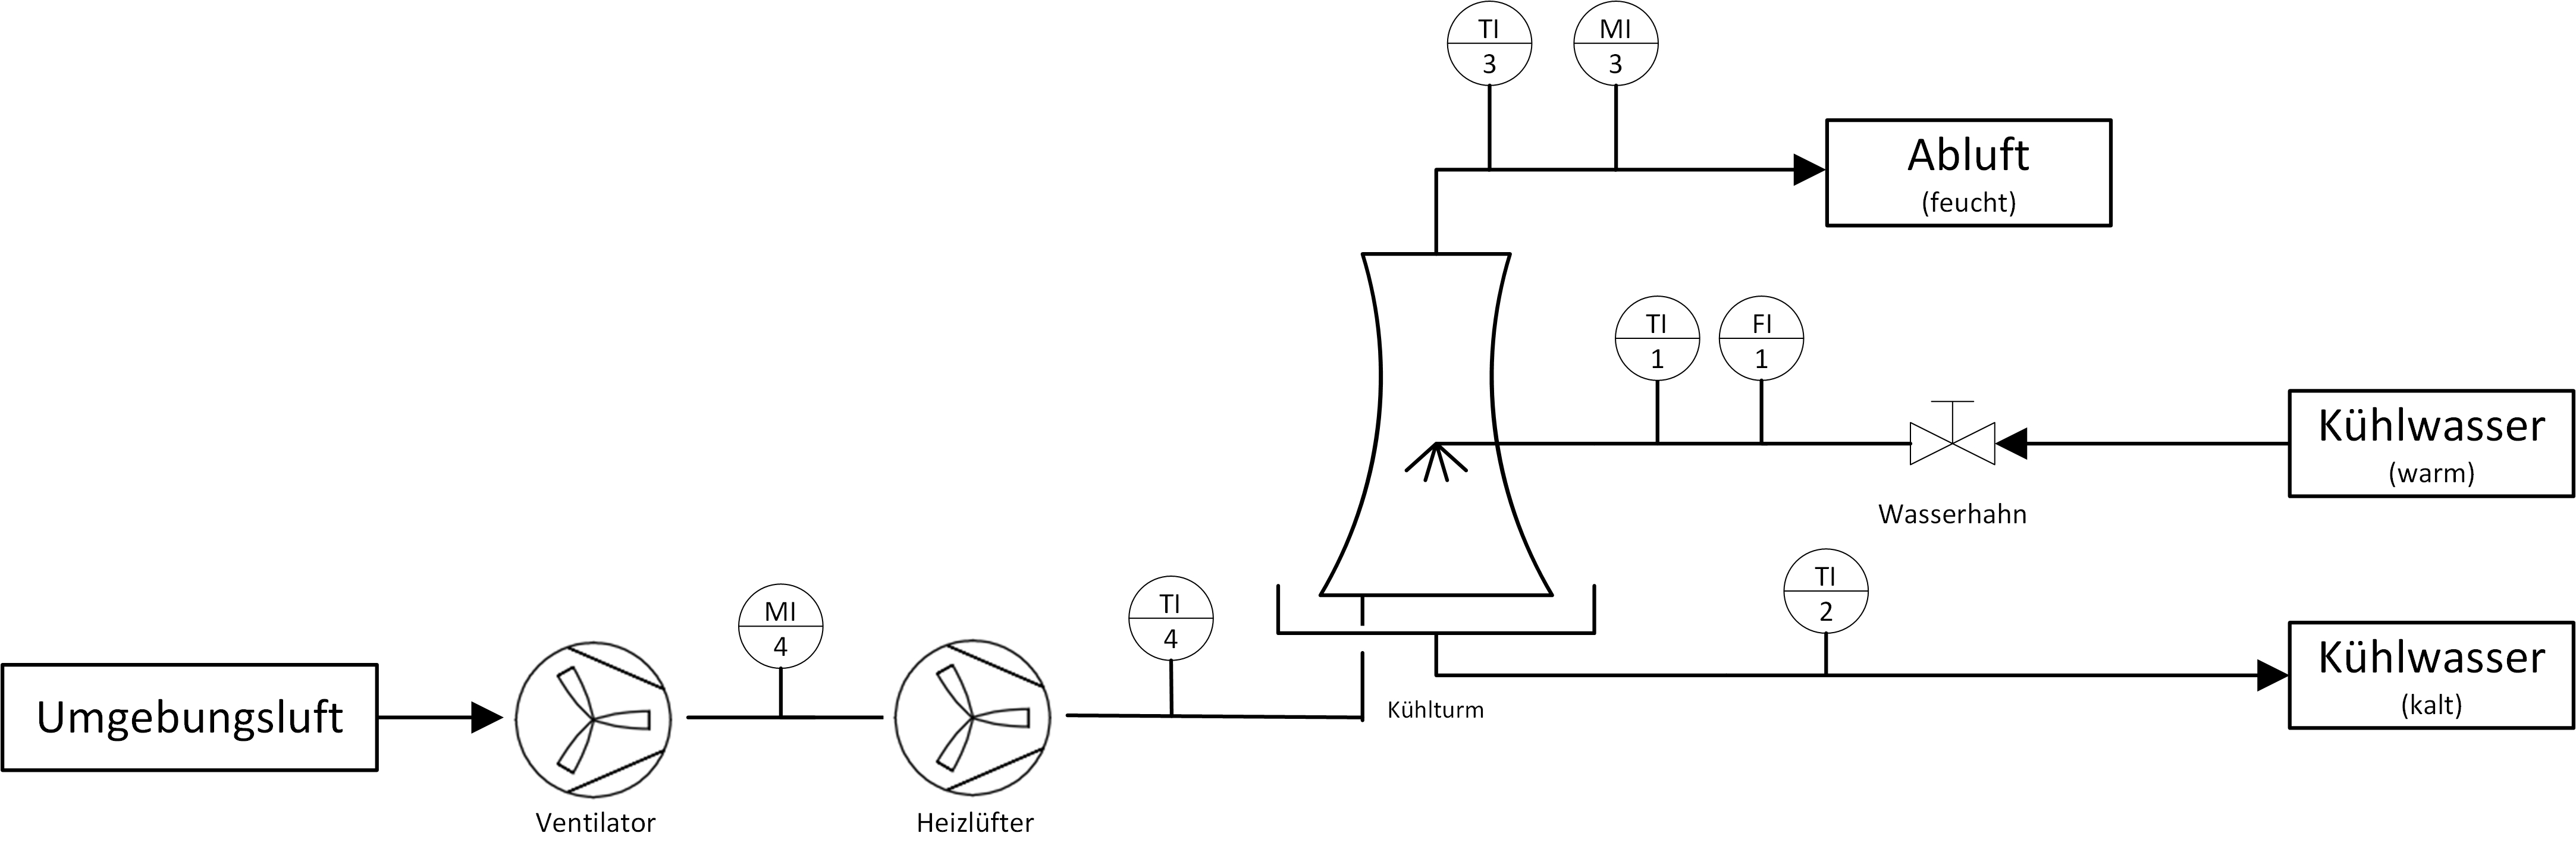
\includegraphics[width=\textwidth]{img/fliessbild}
	\caption{Verfahrensfließbild des Versuchsaufbaus}
	\label{fig:fliessbild}
\end{figure}
\FloatBarrier
%Ende

\subsection*{Durchführung}
Der Versuch gliederte sich in drei Teilversuche, welche sich hauptsächlich in den Betriebsparametern des Versuchsstandes unterscheiden.\\
Begonnen wurde jeweils mit der Bestimmung des Wärmeverlustes des Kühlwassers über die Leitungen. Dafür wurde geprüft, dass die simulierte Luftströmung durch das Gebläse, sowie der Heizlüfter  abgeschaltet waren und lediglich das Kühlwasser den Kühlturm passierte. Dieser Verlustwärmestrom wird für jeden Teilversuch einmal bestimmt  in dem Volumenstrom, Wassereintritts - sowie Wasseraustrittstemperatur gemessen wurden. Innerhalb eines Teilversuches wurde die Wassereingangstemperatur, sowie der Volumenstrom möglichst konstant gehalten.\\
Nun folgten die Messungen der simulierten sommerlichen-Luftströmung im Kühlturm mit dem im Gegenstrom fahrenden warmen Kühlwasser. Es wurde die relative Luftfeuchte nach dem Gebläse und die Temperatur nach dem Heizlüfter der eintretenden Luft gemessen. Beim Austritt aus dem Kühlturm wurde die Luft ebenfalls einer Messung auf relativer Luftfeuchte und Temperatur unterzogen.\\
Um nun unterschiedliche Betriebsparameter zu überprüfen, wurde die eintretende Luft mittels Heizlüfter bei Temperaturen  -\SI{5}{\kelvin}, $\pm$\SI{0}{\kelvin} und +\SI{5}{\kelvin} der Wassereintrittstemperatur eingestellt. Für eine Wassereintrittstemperatur von \SI{35}{\celsius} hätten Lufteingangstemperaturen von \SI{30}{\celsius}, \SI{35}{\celsius} und \SI{40}{\celsius} eingestellt werden müssen.\\
Die Messwerte für Temperatur und relative Feuchte an den verschiedenen Messstellen erfolgten, nach dem schätzungsweise konstante Temperatur über einem Zeitraum von ca. \SI{1}{\minute} an einem externen Computer zu beobachten waren.  Es wurde davon ausgegangen, dass ab diesem Punkt das System stationär fuhr.\\

Für den gesamten Versuch wurde diese Prozedur für Wassereintrittstemperaturen von rund \SI{29}{\celsius}, \SI{38}{\celsius} und \SI{43}{\celsius} durchgeführt.